\chapter{Chaos analysis of the electronic Burridge-Knopoff model}\label{chap: chaos analysis}


\section{Two coupled blocks}\label{sec: 2 blocks chaos}

Relying on the tools that have been introduced in Chapter~\ref{chap: chaos},
it is possible to analyze the chaotic behavior of a system starting from a time series.
Considering the electronic implementation of the Burridge-Knopoff model that has been discussed
in Chapter~\ref{chap: electronic analog of bk}, we can thus analyze the double block behavior
of the circuit (see Section~\ref{sec: double block characterization}).

The time series $y_n$ was chosen to be the signal $W_1$ (see Fig.~\ref{fig: circuit diagram}),
which was sampled for 10 s with a sampling time of 0.1 ms, resulting in $10^5$ points in the sequence.
The driving voltage $V_d$ was set to 0.05 V, since the chaotic behavior seems present only for
$V_d \lesssim 0.11$ V (see Fig.~\ref{fig: bifurcation}). The results of the application of the
``chasing chaos'' method described in Section~\ref{sec: method for chaos} are shown in Fig.~\ref{fig:2 blocks chaos}.

\begin{figure}[ht!]
    \centering
    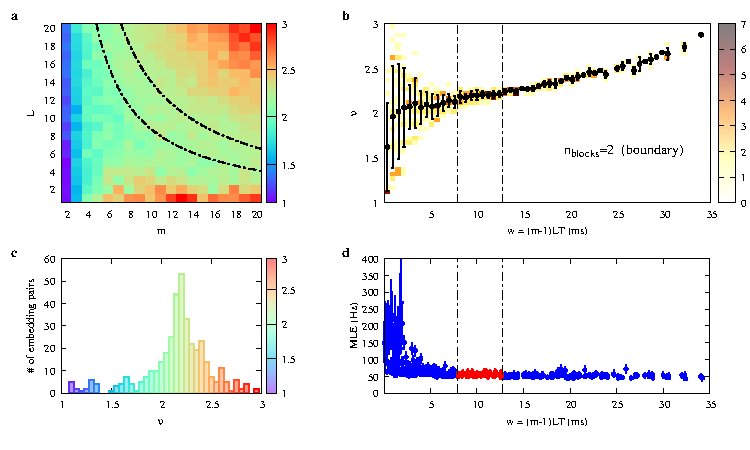
\includegraphics[width=\linewidth]{../blocks/2_blocks/1e5_points/plots/chaos.pdf}
    \caption{``Chasing chaos'' analysis of the experimental $W_1$ time series
    obtained by setting $V_d=0.05$ V with 2 coupled blocks.
    The number of elements in the sequence is $10^5$.
    (a) Map of estimated correlation dimension $\nu$ vs.\ embedding pair $(m, L)$.
    The black, dash-dotted hyperbolae bound the region of uniform $\nu$ corresponding to the interval of the
    embedding window $w$ highlighted in (b) and (d).
    (b) Sample joint distribution of $(w,\nu)$ for the $\nu$-map in (a).
    Black dots and the related errobars correspond to the expected value and the related uncertainty of $\nu$
    for each given value (bin) of $w$. A uniformity region, highlighted by the dash-dotted vertical lines,
    is identified. (c) Histogram of the estimated $\nu$. (d) Distribution of MLE as a function of $w$. Each point and the related
    uncertainty corresponds to the value assessed on an embedding pair by using the divergence rate method.
    A cluster of points, marked in red, can be identified in the uniformity region of (b), also highlighted here.
    }\label{fig:2 blocks chaos}
\end{figure}

In Fig.~\ref{fig:2 blocks chaos}a the heatmap of the correlation dimension $\nu$ in the embedding
lattice is shown. The two hyperbolae bound the uniformity region, which was chosen by searching for
a plateau in the joint distribution in Fig.~\ref{fig:2 blocks chaos}b.
Carrying out a weighted average of the correlation dimension estimates in the uniformity region yields
$\nu=2.20\pm0.02$, which complies with the peak of the histogram in Fig.~\ref{fig:2 blocks chaos}c,
which is $2.20\pm0.05$.

The estimates of the maximum Lyapunov exponent as a function of the embedding window are shown in
Fig.~\ref{fig:2 blocks chaos}d. Carrying out another weighted average of the MLE in the uniformity region
yields $\text{MLE}=(54\pm1)$ Hz. Since the uniformity region is easy to be identified, it is reasonable
to conclude that this system is chaotic.
Nonetheless, the estimates of $\nu$ and MLE are assumed to be valid.

This chaos analysis was carried out also on a breadboard implementation of the circuit~\cite{ref:electronic_analog}.
A uniformity region was identified and the correlation dimension was found to be
$\nu=1.971\pm0.007$. Regarding the MLE, a cluster of values at about 45 Hz occurred, which complied
with the numerical value $\text{MLE}=(46\pm5)$ Hz, which was found integrating the differential
equations of the system (Eq.~\ref{eq: 2 block motion electronic}) and applying the so-called
standard method~\cite{benettin1980lyapunov1,benettin1980lyapunov2}.

Both the estimates for the correlation dimension and the maximum Lyapunov exponent are larger
in the integrated board case with respect to the breaboard case.
A possible explanation for this is the higher presence of noise in the integrated board;
as was discussed in Section~\ref{subsec: testing the procedure}, the correlation dimension evaluation
increases with noise.

Nevertheless, the chaotic dynamics is observed in both implementations. The calculations of $\nu$ and
MLE strongly depend on many factors, such as the embedding lattice, the sampling time, or the
arbitrariness on the choice of the uniformity region.
Thus, the results on the two implementations are assumed to be in compliance with each other.


\section{Three coupled blocks}\label{sec: 3 blocks chaos}

After establishing that the system constituted of two coupled blocks is chaotic, it can be interesting
to observe what happens when more than two blocks are coupled, starting for now from three.
In particular, assuming that the chaotic behavior is preserved, the interesting part is the dependence
of $\nu$ and MLE on the number of coupled blocks.

Something to be considered when dealing with three or more coupled blocks is the choice of the time series.
In the two blocks case, choosing $W_1$ or $W_2$ was perfectly equivalent.
In the three blocks case, instead, we can distinguish between blocks on the ``boundary'' (block 1 and
block 3) and blocks in the ``center'' (block 2). Takens' theorem~\cite{ref:takens2006detecting}
states that the results of the embedding procedure should be independent of the choice of the state
variable; once again, this is true for noiseless, finely sampled and infinitely long sequences.
It is thus reasonable to perform the analysis in both cases.


\subsection{Block on the boundary}\label{subsec: 3 blocks chaos boundary}

The time series $y_n$ was chosen to be the signal $W_1$ (block on the boundary),
which was sampled for 10 s with a sampling time of 0.1 ms, resulting in $10^5$ points in the sequence.
The driving voltage $V_d$ was kept at 0.05 V. The results of the application of the
``chasing chaos'' method are shown in Fig.~\ref{fig:3 blocks chaos boundary 1e5}.

\begin{figure}[ht!]
    \centering
    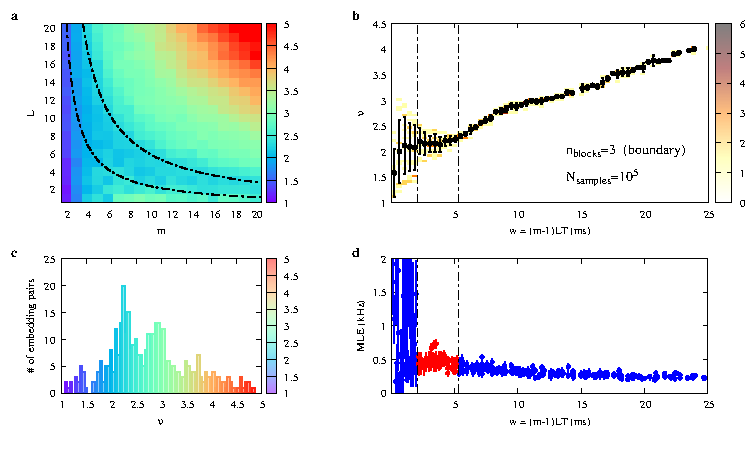
\includegraphics[width=\linewidth]{../blocks/3_blocks/edge/1e5_points/plots/chaos_low.pdf}
    \caption{``Chasing chaos'' analysis of the experimental $W_1$ time series obtained by setting $V_d=0.05$ V with 3 coupled blocks.
    The number of elements in the sequence is $10^5$.
    (a) Map of estimated correlation dimension $\nu$ vs.\ embedding pair $(m, L)$.
    The black, dash-dotted hyperbolae bound the region of uniform $\nu$ corresponding to the interval of the
    embedding window $w$ highlighted in (b) and (d).
    (b) Sample joint distribution of $(w,\nu)$ for the $\nu$-map in (a).
    Black dots and the related errobars correspond to the expected value and the related uncertainty of $\nu$
    for each given value (bin) of $w$. A uniformity region, highlighted by the dash-dotted vertical lines,
    is identified. (c) Histogram of the estimated $\nu$. (d) Distribution of MLE as a function of $w$. Each point and the related
    uncertainty corresponds to the value assessed on an embedding pair by using the divergence rate method.
    A cluster of points, marked in red, can be identified in the uniformity region of (b), also highlighted here.
    }\label{fig:3 blocks chaos boundary 1e5}
\end{figure}

Using the same methods employed in the previous section, the correlation dimension averaged on the
uniformity region yields $\nu=2.21\pm0.04$, which complies with the histogram peak
which is at $2.25\pm0.05$. The maximum Lyapunov exponent in the uniformity region was found 
to be equal to $\text{MLE}=(453\pm6)$ Hz.

The system is once again chaotic, and both $\nu$ and MLE have increased with respect to the values found
in the two blocks case. In particular, while the increment of the correlation dimension is small, the
MLE changes by an order of magnitude. This might hint to the fact that $\nu$ depends linearly on the
number of coupled blocks, while the MLE has an exponential dependence; this will be unraveled
in Section~\ref{sec: many blocks chaos}.

Something that should be taken into account is that the choice on the sampling time might be improved.
The reason for this is that the uniformity region is found at very small values of the embedding
window (see Fig.~\ref{fig:3 blocks chaos boundary 1e5}) with respect to the total time spanned
by the embedding lattice. This means that reducing the sampling time might increase the number of
points in the uniformity region, thus improving the estimates on $\nu$ and MLE\@.

Another ``chasing chaos'' analysis was then carried out by setting the sampling time to 0.05 ms,
doubling the number of elements in the time series, i.e.\ $2\times10^5$.
The results are shown in Fig.~\ref{fig:3 blocks chaos boundary 2e5}.

\begin{figure}[ht!]
    \centering
    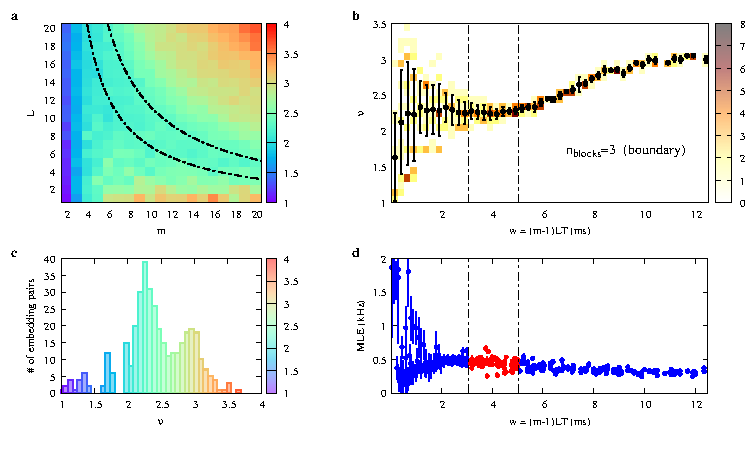
\includegraphics[width=\linewidth]{../blocks/3_blocks/edge/2e5_points/plots/chaos_low.pdf}
    \caption{``Chasing chaos'' analysis of the experimental $W_1$ time series obtained by setting $V_d=0.05$ V with 3 coupled blocks.
    The number of elements in the sequence is $2\times10^5$.
    (a) Map of estimated correlation dimension $\nu$ vs.\ embedding pair $(m, L)$.
    The black, dash-dotted hyperbolae bound the region of uniform $\nu$ corresponding to the interval of the
    embedding window $w$ highlighted in (b) and (d).
    (b) Sample joint distribution of $(w,\nu)$ for the $\nu$-map in (a).
    Black dots and the related errobars correspond to the expected value and the related uncertainty of $\nu$
    for each given value (bin) of $w$. A uniformity region, highlighted by the dash-dotted vertical lines,
    is identified. (c) Histogram of the estimated $\nu$. (d) Distribution of MLE as a function of $w$. Each point and the related
    uncertainty corresponds to the value assessed on an embedding pair by using the divergence rate method.
    A cluster of points, marked in red, can be identified in the uniformity region of (b), also highlighted here.
    }\label{fig:3 blocks chaos boundary 2e5}
\end{figure}

The new estimate for the correlation dimension yields $\nu=2.27\pm0.02$, which complies with the
histogram peak which is at $2.260\pm0.035$. The maximum Lyapunov exponent in the uniformity region was found 
to be equal to $\text{MLE}=(439\pm4)$ Hz.

These estimates are very similar to the results obtained with $10^5$ points.
Nonetheless, the errors have slightly been improved, and the plateau is more visible and contains
more points. This change in the sampling time will be much more relevant when dealing with systems
with many coupled blocks.


\subsection{Block in the center}\label{subsec: 3 blocks chaos center}

The chaos analysis was then carried out on the time series obtained by sampling the signal $W_2$
(block in the center) with a sampling time of 0.05 ms, resulting in $2\times10^5$ elements of the
sequence. The results are shown in Fig.~\ref{fig:3 blocks chaos center 2e5}.

\begin{figure}[ht!]
    \centering
    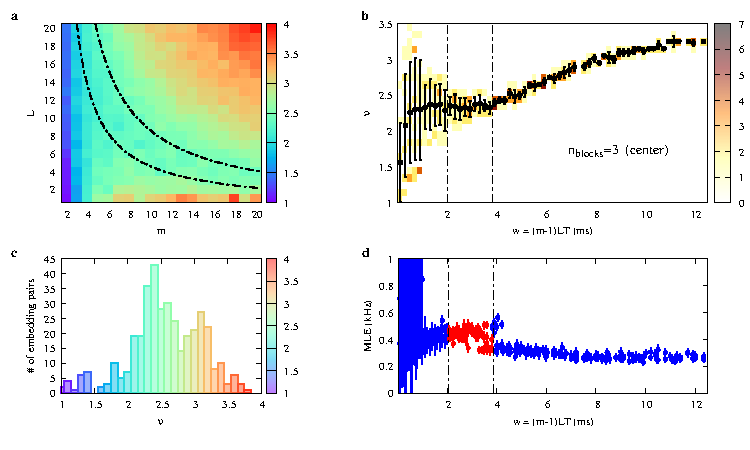
\includegraphics[width=\linewidth]{../blocks/3_blocks/middle/2e5_points/plots/chaos_low.pdf}
    \caption{``Chasing chaos'' analysis of the experimental $W_2$ time series obtained by setting $V_d=0.05$ V with 3 coupled blocks.
    The number of elements in the sequence is $2\times10^5$.
    (a) Map of estimated correlation dimension $\nu$ vs.\ embedding pair $(m, L)$.
    The black, dash-dotted hyperbolae bound the region of uniform $\nu$ corresponding to the interval of the
    embedding window $w$ highlighted in (b) and (d).
    (b) Sample joint distribution of $(w,\nu)$ for the $\nu$-map in (a).
    Black dots and the related errobars correspond to the expected value and the related uncertainty of $\nu$
    for each given value (bin) of $w$. A uniformity region, highlighted by the dash-dotted vertical lines,
    is identified. (c) Histogram of the estimated $\nu$. (d) Distribution of MLE as a function of $w$. Each point and the related
    uncertainty corresponds to the value assessed on an embedding pair by using the divergence rate method.
    A cluster of points, marked in red, can be identified in the uniformity region of (b), also highlighted here.
    }\label{fig:3 blocks chaos center 2e5}
\end{figure}

The estimates for the correlation dimension and the maximum Lyapunov exponent yield
$\nu=2.34\pm0.04$ and $\text{MLE}=(427\pm4)$ Hz.
While the MLE is practically the same as the boundary case, the correlation dimension is slightly
larger; the uncertainty on $\nu$ is also increased.
In order to make a guess on the reasons why
this discrepancy occurs it is necessary to consider the oscilloscope quantization,
as will be done in the following section.

The difference between the two cases can also be appreciated by looking at the attractor plots,
shown in Fig.~\ref{fig: 3 blocks attractors}. The signals taken from the center block seems to be
``more chaotic'', in the sense that the phase space is explored more in the same amount of time.
Intuitively, since the block in the center is linked to two blocks instead of one, it seems reasonable
that the signal is, once again, ``more chaotic''.
However, this should not modify the estimates of $\nu$ and MLE, since $W_2$ and $W_1$ are both
variables of the same system of differential equations. This means that there is some
``experimental'' reason for which this strange behavior is observed.

\begin{figure}[ht!]
    \centering
    \subfloat{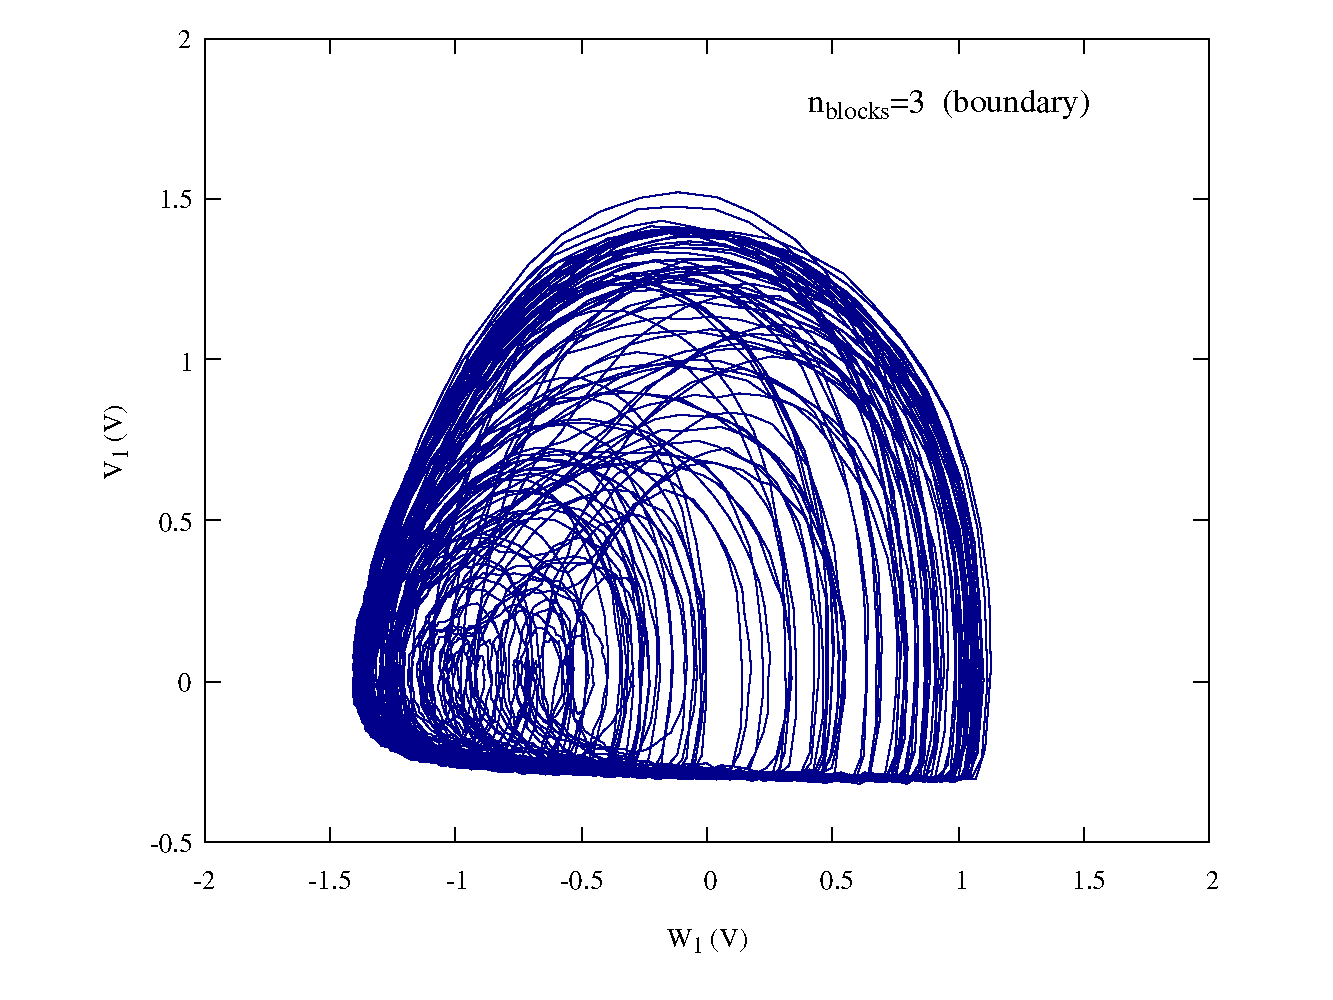
\includegraphics[width=0.47\linewidth]{../blocks/3_blocks/edge/attractor.pdf}}
    \subfloat{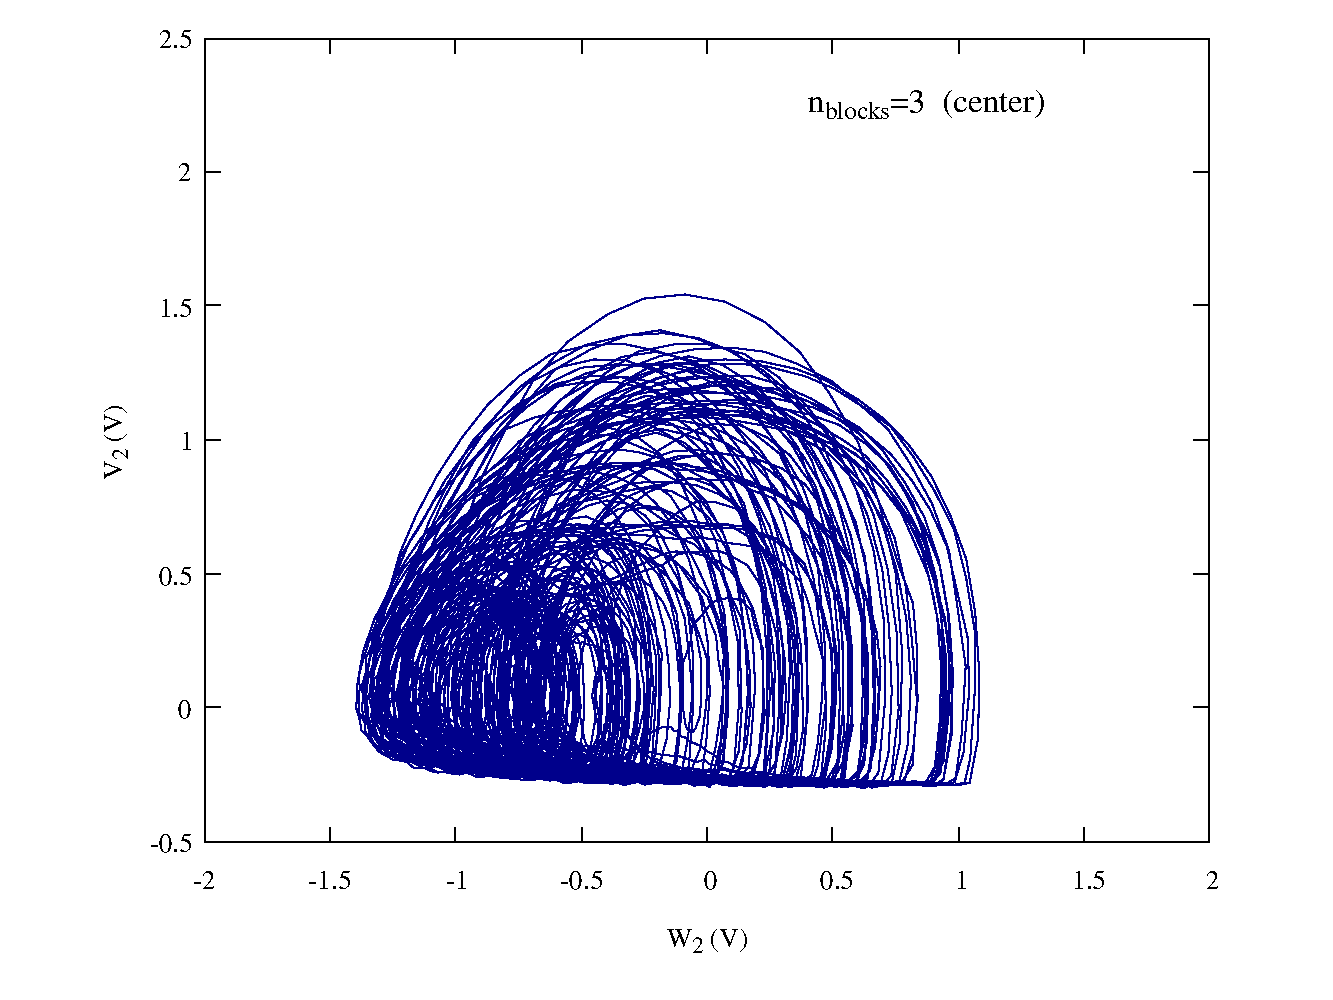
\includegraphics[width=0.47\linewidth]{../blocks/3_blocks/middle/attractor.pdf}}
    \caption{Phase portraits of $V$ vs $W$ for 3 coupled blocks, analyzing the block on the boundary
    (left) and in the center (right), for a total time of 5 s, setting $V_d=0.05$ V.
    }\label{fig: 3 blocks attractors}  
\end{figure}


\section{The effects of the oscilloscope quantization}\label{sec: oscilloscope quantization}
%CONTROLLA I BIT DELL'OSCILLOSCOPIOOOOOOOOOOOOOOOOOOOOOOOOOOOOOOOOOOOO!!!!!!!!!!!!!!!!!!!!
One of the possible reasons for which the results of the chaos analysis differ between $W_1$ and $W_2$
might lay in the quantization of the oscilloscope, with which the signals are sampled.
The data read by the oscilloscope are stored in a finite number of bits, namely eight.
When dealing with chaotic signals, i.e.\ with sharp peaks and rapid changes of the signal,
this quantization reduces the information given by a time series; moreover, it can introduce
spurious contributions that can modify the estimates on the correlation dimension and the maximum
Lyapunov exponent.

In order to test the actual effects of this quantization on the analysis, the following method was
employed.
\begin{itemize}
    \item
    Given the signal $y_n$, the smallest separation between two successive elements
    $y_n,y_{n+1}$, i.e.\ the oscilloscope quantization, is searched for.
    For example, if the signal is:
    \begin{equation*}
        \{y_n\}=(1.5,\,1.5,\,1.75,\,2,\,2.5,\,2.75),
    \end{equation*}
    the quantization is 0.25.

    \item
    The signal is then divided by the quantization, so that each element becomes an integer
    ($y_n\rightarrow y_n^{\text{int}}$).
    In the example, the signal $y_n$ becomes:
    \begin{equation*}
        \{y_n^{\text{int}}\}=\left\{\frac{y_n}{0.25}\right\}=(6,\,6,\,7,\,8,\,10,\,11).
    \end{equation*}

    \item
    Then an integer division is performed on the signal, i.e.\ $y_n^{\text{int}}$ is first divided
    by two, then rounded to the lowest integer and multiplied by two again
    ($y_n^{\text{int}}\rightarrow \tilde{y}_n^{\text{int}}$).
    Our example sequence then becomes:
    \begin{equation*}
        \{\tilde{y}_n^{\text{int}}\}=(6,\,6,\,6,\,8,\,10,\,10).
    \end{equation*}

    \item
    In the end, the resulting sequence is multiplied by the quantization, so that:
    \begin{equation*}
        \{\tilde{y}_n\}=(1.5,\,1.5,\,1.5,\,2,\,2.5,\,2.5).
    \end{equation*}
\end{itemize}

The time series $\{\tilde{y}_n\}$ obtained at the end of this process is very similar to the
the starting sequence $y_n$, with the difference that the quantization is doubled.
Therefore, carrying out the chasing chaos analysis on both sequences should give an idea on the
effect of the quantization on the estimates of $\nu$ and MLE\@.

The analysis was then carried out on the system of four coupled blocks.
The starting signal was chosen to be $W_1$, from which the double quantized signal $\tilde{W}_1$
was obtained. In order to improve the reasoning, also the quadrupled quantized signal $\tilde{\tilde{W}}_1$
was analyzed. The graphical results of these analyses are shown in Appendix~\ref{app: quantization}.
The estimates of $\nu$ and MLE in the three cases are presented in Table~\ref{tab: quantization}.

% chktex-file 44
\begin{table}[ht!]
    \centering
    \begin{tabular}{c|c|c}
                    & $\nu$         & MLE (kHz)     \\ \hline
        $W_1$       & $2.29\pm0.03$   & $1.03\pm0.04$ \\ \hline
        $\tilde{W}_1$ & $2.36\pm0.06$   & $1.05\pm0.05$ \\ \hline
        $\tilde{\tilde{W}}_1$ & $2.54\pm0.11$ & $0.87\pm0.06$
    \end{tabular}
    \caption{Estimates of $\nu$ and MLE on the system of four coupled blocks.
    $W_1$ is the signal given by the oscilloscope, while $\tilde{W}_1$ and $\tilde{\tilde{W}}_1$ are
    obtained from $W_1$ by doubling and quadrupling the quantization, respectively.
    }\label{tab: quantization}
\end{table}

The MLE is not too sensible to the oscilloscope quantization, since it has an observable decrease
only in the quadrupled quantization case. On the other hand, both the correlation dimension and
its uncertainty significantly increase with the quantization.
This results are consistent with the discrepancies found in the three blocks case between
the boundary block and the center block, hinting to the fact that the oscilloscope quantization
might play a compelling role in the chaos analysis.


\section{Multiple coupled blocks}\label{sec: many blocks chaos}

It is now possible to fully utilize the integrated board, coupling an arbitrary number
of blocks and studying the chaotic dynamics that comes with it.
In particular, the chaos analysis was carried out with the number of coupled blocks ranging from
2 to 25, always choosing $W_1$ as the time series, i.e.\ a block on the boundary.
When the number of coupled blocks was odd, an additional analysis was carried out on the signal $W_k$,
where the $k$-th block is located in the center (e.g.\ in the 7 blocks case,
the analyzed signal will be $W_4$). The driving voltage was always set equal to 0.05 V, and the
number of elements in the sequence was always kept at $2\times10^5$.
The graphical results of these analyses are shown in Appendix~\ref{app: multiple blocks}.

The correlation dimension and the maximum Lyapunov exponent as a function of the number of coupled
blocks are shown in Fig.~\ref{fig:nu mle blocks} for both the boundary blocks and the center blocks.

\begin{figure}[ht!]
    \centering
    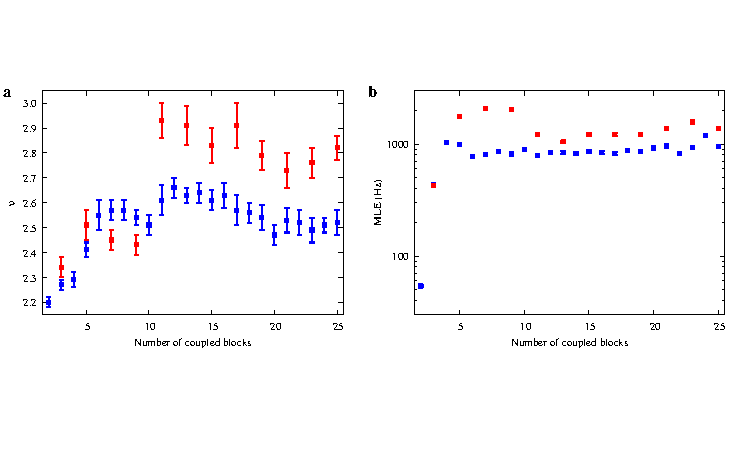
\includegraphics[width=\linewidth,trim={0 1.5cm 0 1.3cm},clip]
    {../blocks/data/nu_mle_blocks.pdf}
    \caption{Correlation dimension (a) and maximum Lyapunov exponent (b) estimates
    as a function of the number of coupled blocks. The blue points represent blocks on the boundary,
    while the red ones represent blocks in the center.}\label{fig:nu mle blocks}
\end{figure}

The correlation dimension of the boundary blocks increases noticeably fast up until 6 coupled blocks,
from which $\nu$ seems to fluctuate around a plateau value $\nu_{\text{pl}}=2.56\pm0.01$, which was
obtained from a weighted average of the $\nu$ values from 6 to 25 coupled blocks.

Regarding the center blocks instead, the majority of the $\nu$ values are larger with respect to the
corresponding estimates on the boundary blocks, and the same goes for the uncertainties.
A possible reason for this behavior can be once again the oscilloscope quantization.
As can be seen from the attractor plots in Fig.~\ref{fig:attractors 11-17}, the explored region
of the phase space is smaller when looking at center blocks.
This means that the oscilloscope quantization is more relevant in this case, resulting in higher
estimates of the correlation dimension.

\begin{figure}[ht!]
    \centering
    \begin{minipage}{.47\textwidth}
        \begin{subfigure}{\linewidth}
            \centering
            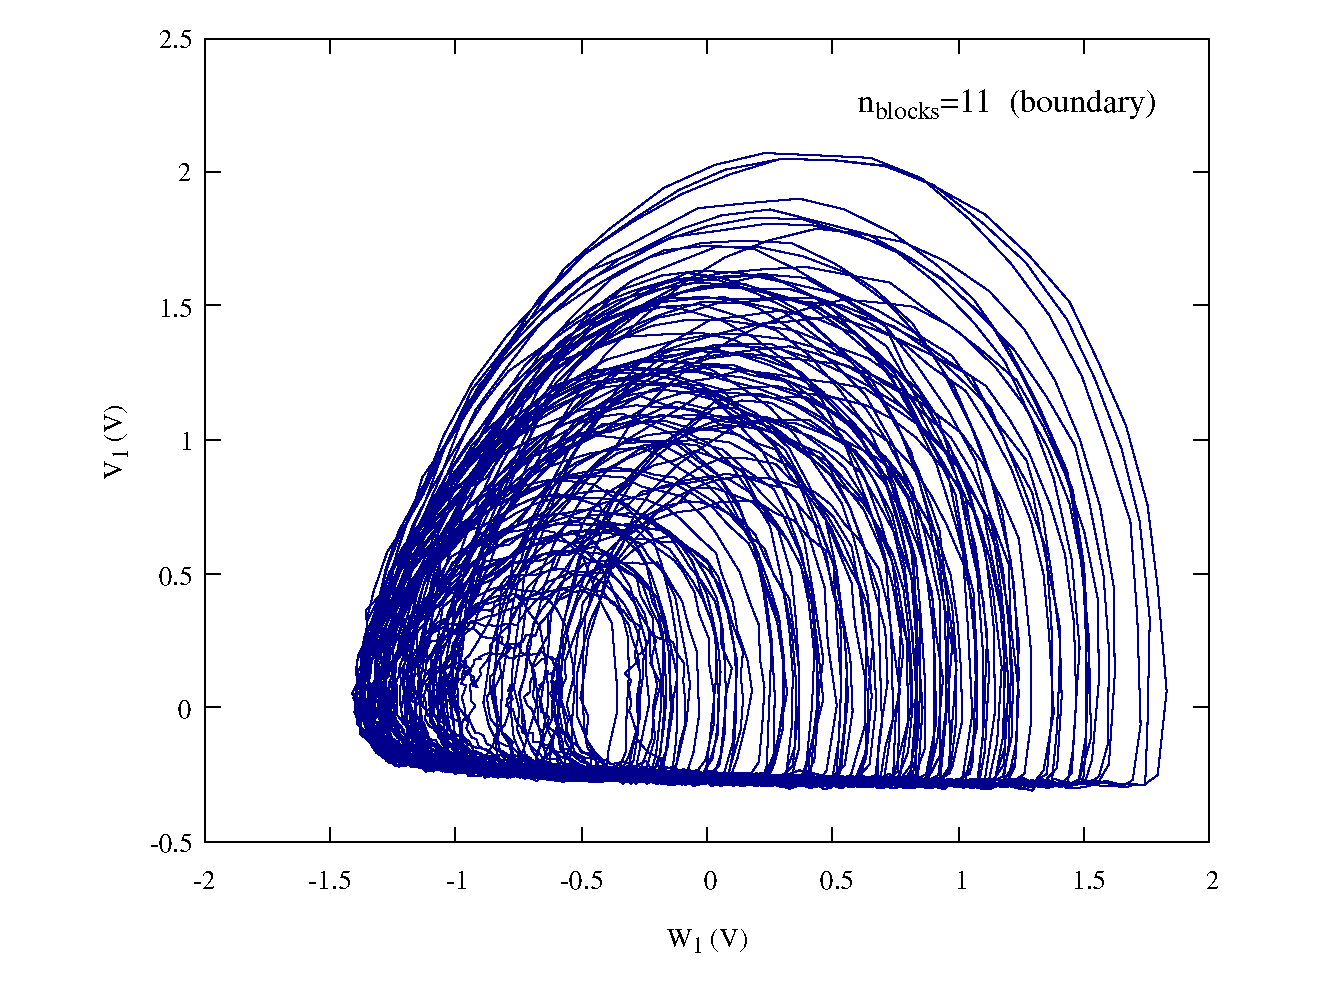
\includegraphics[width=\linewidth]
            {../blocks/11_blocks/edge/attractor.pdf}
        \end{subfigure}
    \end{minipage}
    \begin{minipage}{.47\textwidth}
        \begin{subfigure}{\linewidth}
            \centering
            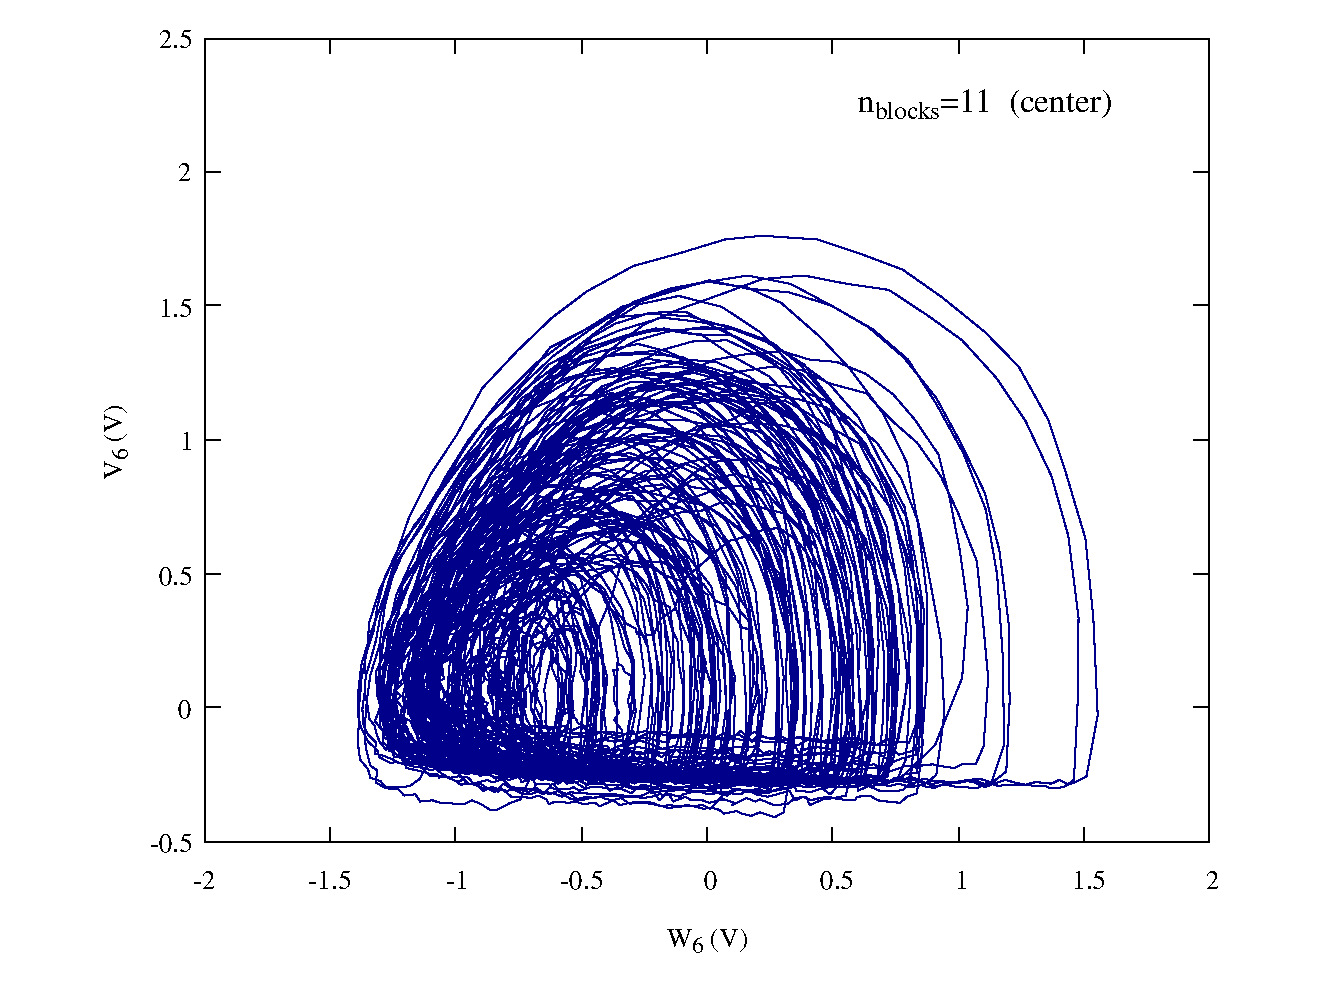
\includegraphics[width=\linewidth]
            {../blocks/11_blocks/middle/attractor.pdf}
        \end{subfigure}
    \end{minipage}
    \begin{minipage}{.47\textwidth}
        \begin{subfigure}{\linewidth}
            \centering
            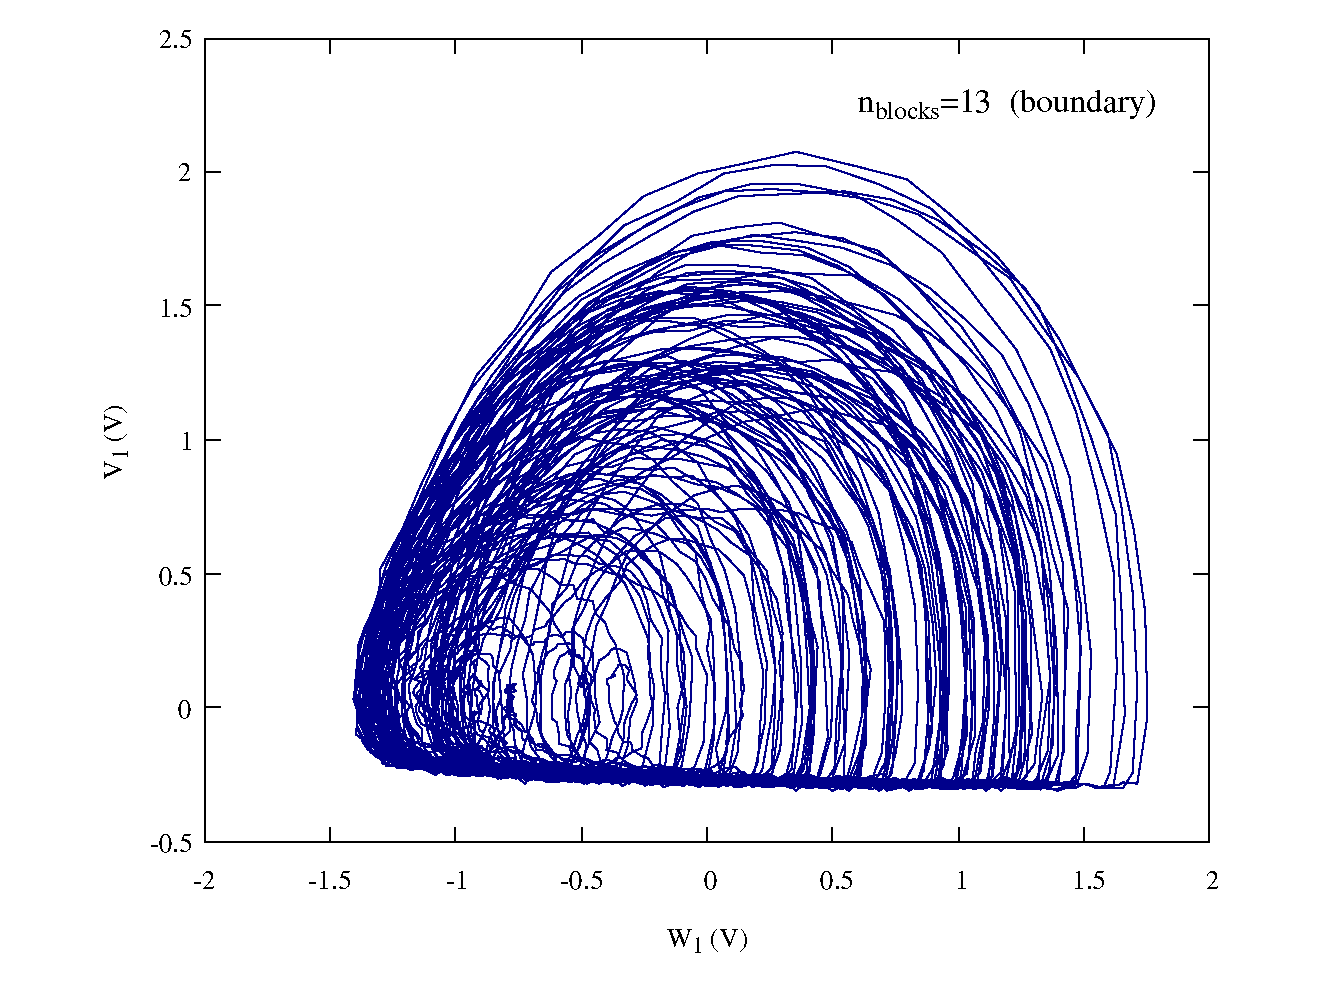
\includegraphics[width=\linewidth]
            {../blocks/13_blocks/edge/attractor.pdf}
        \end{subfigure}
    \end{minipage}
    \begin{minipage}{.47\textwidth}
        \begin{subfigure}{\linewidth}
            \centering
            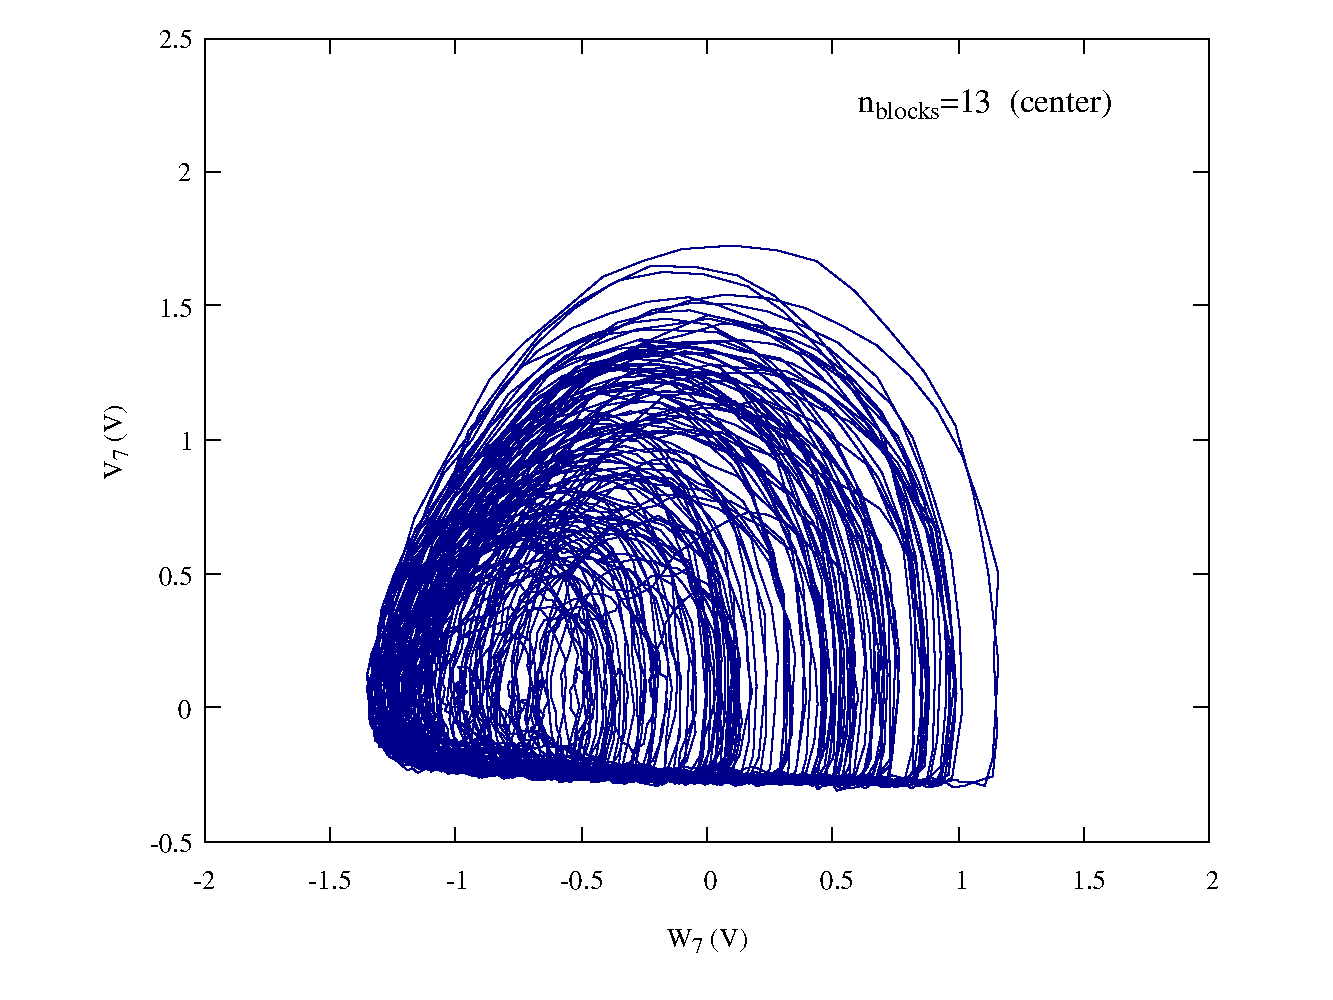
\includegraphics[width=\linewidth]
            {../blocks/13_blocks/middle/attractor.pdf}
        \end{subfigure}
    \end{minipage}
    \begin{minipage}{.47\textwidth}
        \begin{subfigure}{\linewidth}
            \centering
            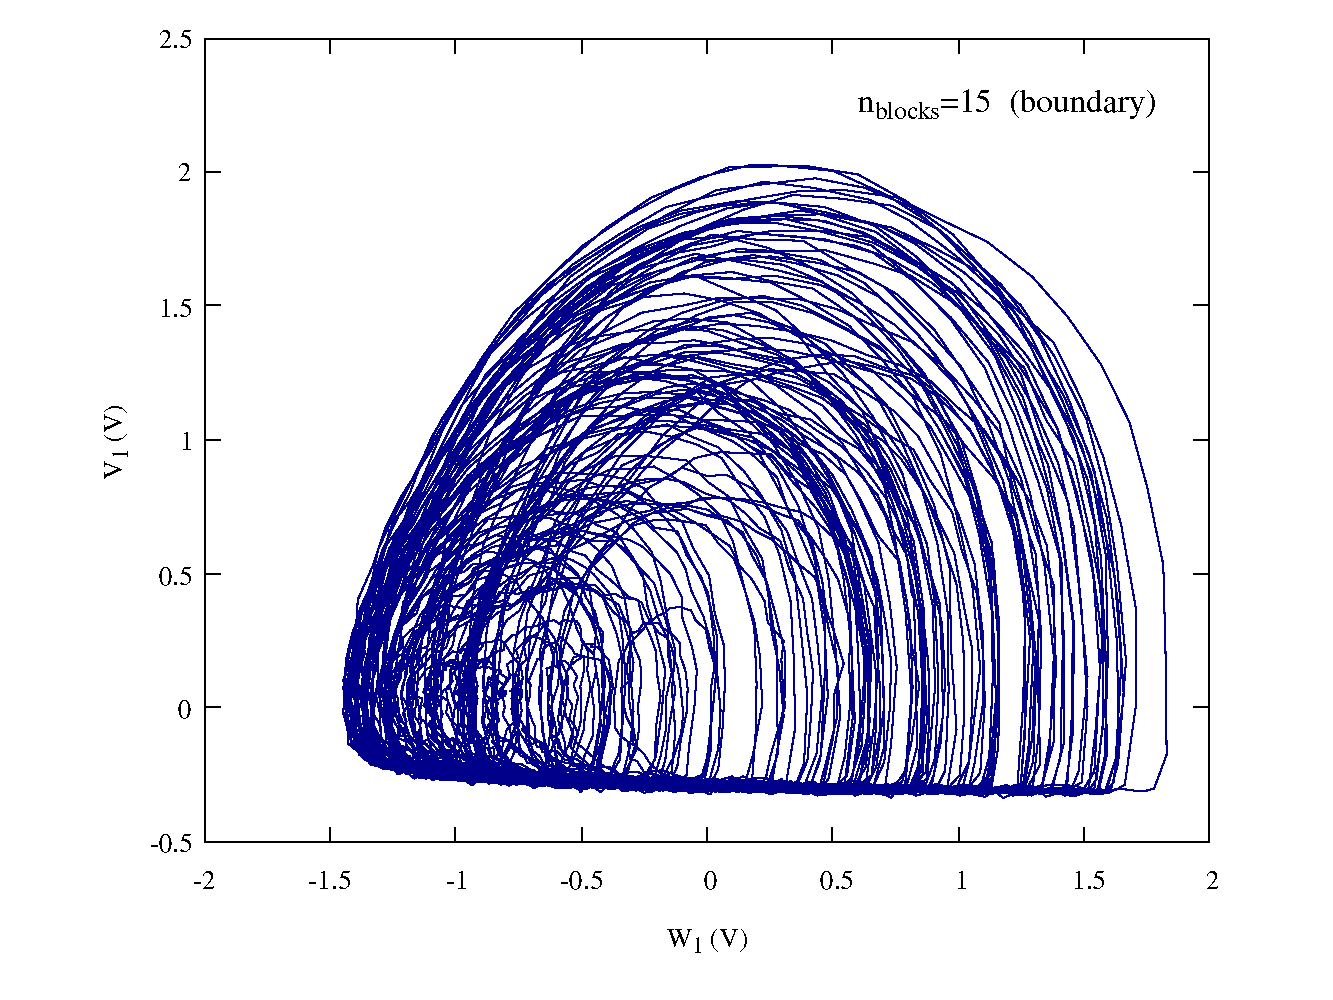
\includegraphics[width=\linewidth]
            {../blocks/15_blocks/edge/attractor.pdf}
        \end{subfigure}
    \end{minipage}
    \begin{minipage}{.47\textwidth}
        \begin{subfigure}{\linewidth}
            \centering
            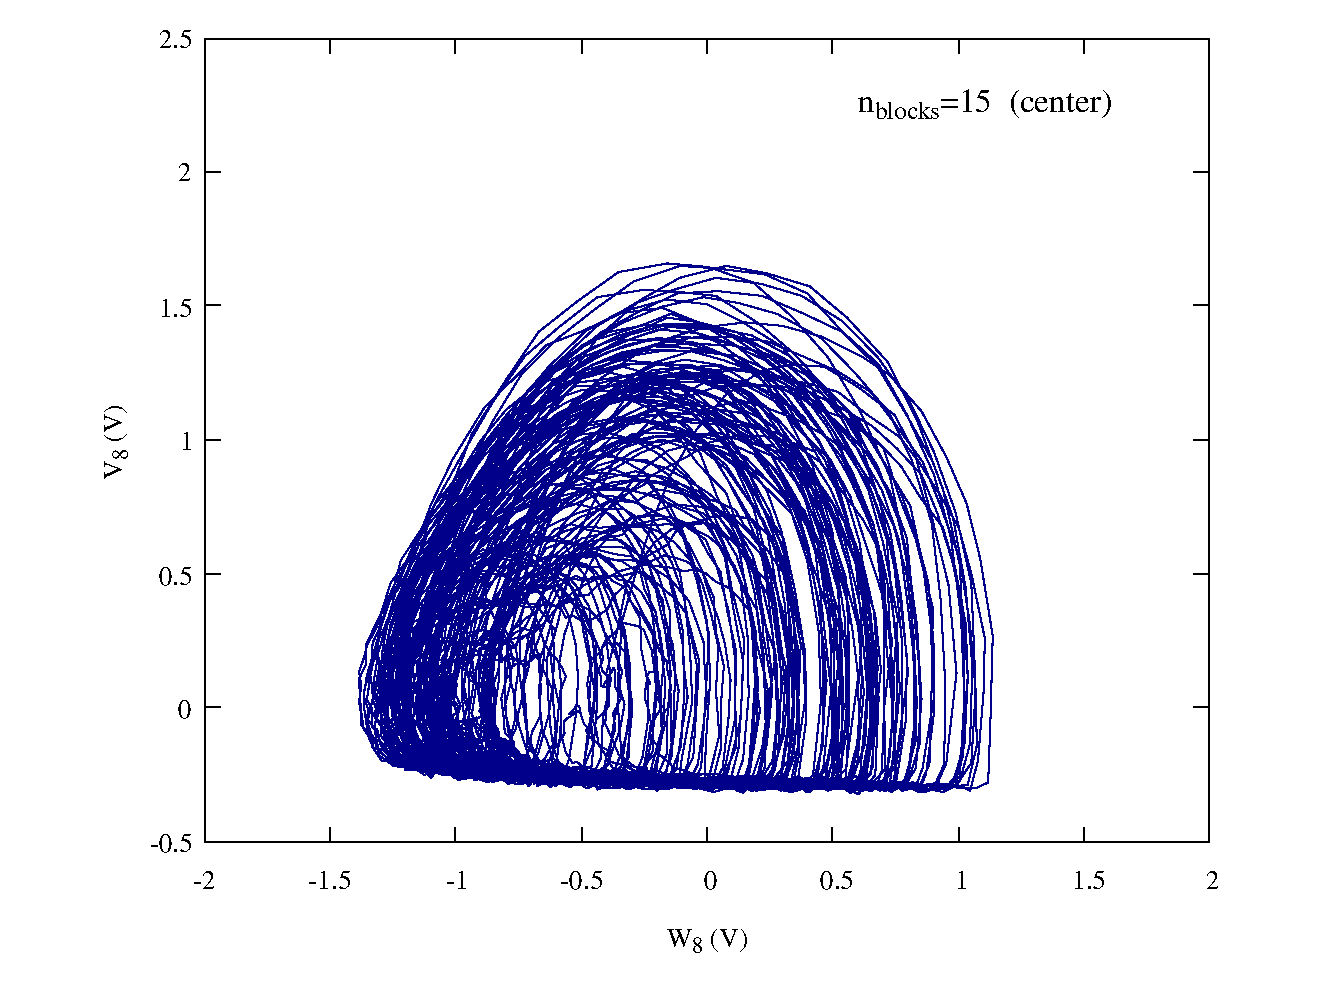
\includegraphics[width=\linewidth]
            {../blocks/15_blocks/middle/attractor.pdf}
        \end{subfigure}
    \end{minipage}
    \begin{minipage}{.47\textwidth}
        \begin{subfigure}{\linewidth}
            \centering
            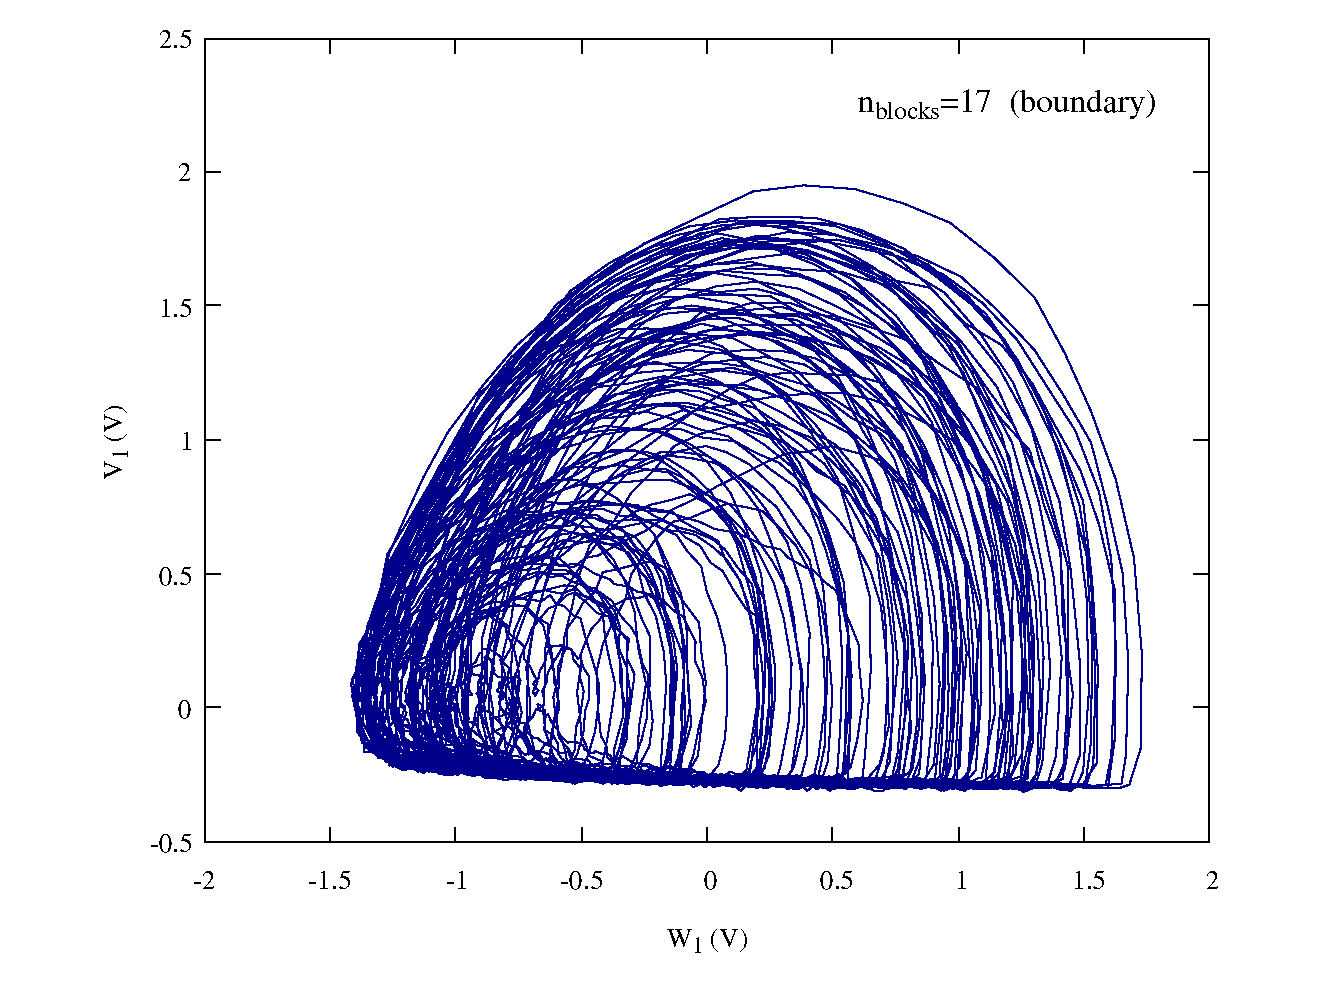
\includegraphics[width=\linewidth]
            {../blocks/17_blocks/edge/attractor.pdf}
        \end{subfigure}
    \end{minipage}
    \begin{minipage}{.47\textwidth}
        \begin{subfigure}{\linewidth}
            \centering
            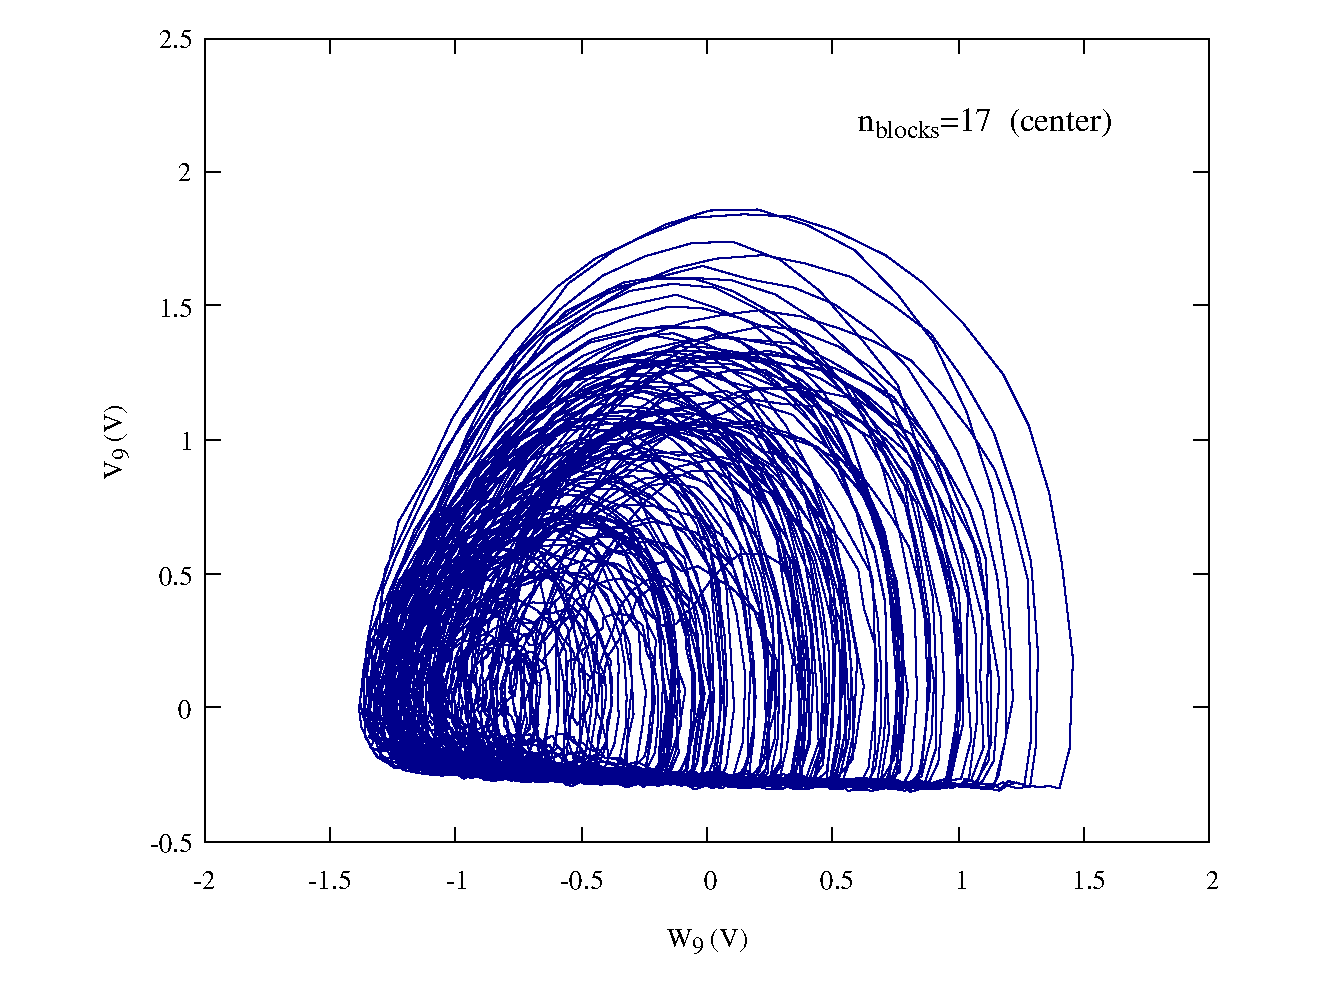
\includegraphics[width=\linewidth]
            {../blocks/17_blocks/middle/attractor.pdf}
        \end{subfigure}
    \end{minipage}
    \caption{Phase portraits of $V$ vs $W$ from 11 to 17 coupled blocks, analyzing the block on the boundary
    (left) and in the center (right), for a total time of 5 s, setting $V_d=0.05$ V.}\label{fig:attractors 11-17}
\end{figure}

Regarding the maximum Lyapunov exponent for the boundary blocks, its rapid increase stops at 4 coupled
blocks, from which it starts fluctuating around a plateau of about 865 Hz.
Once again, the MLE values estimated using the center blocks are larger than the boundary ones.
This cannot be explained with the oscilloscope quantization, since the dependence of the MLE on
it is very weak; moreover, the MLE should decrease with the quantization, while here it increases.

An important consideration in this regard is the following. In Fig.~\ref{fig: 13 blocks chaos boundary}
and Fig.~\ref{fig: 13 blocks chaos center}
the results of the chaos analysis for 13 coupled blocks are shown, for the boundary and center case
respectively.

\begin{figure}[ht!]
    \centering
    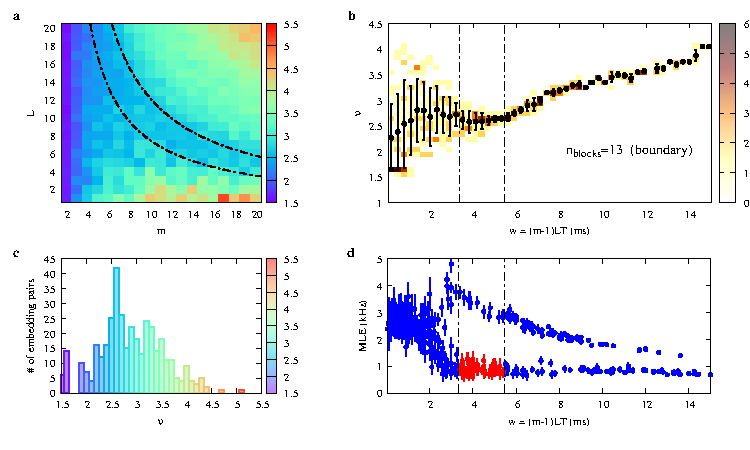
\includegraphics[width=\linewidth]{../blocks/13_blocks/edge/2e5_points/plots/chaos_low.pdf}
    \caption{``Chasing chaos'' analysis of the experimental $W_1$ time series with 13 coupled blocks.
    (a) Map of estimated correlation dimension $\nu$ vs.\ embedding pair $(m, L)$.
    (b) Sample joint distribution of $(w,\nu)$ for the $\nu$-map in (a).
    (c) Histogram of the estimated $\nu$. (d) Distribution of MLE as a function of $w$.
    }\label{fig: 13 blocks chaos boundary}
\end{figure}

\begin{figure}[ht!]
    \centering
    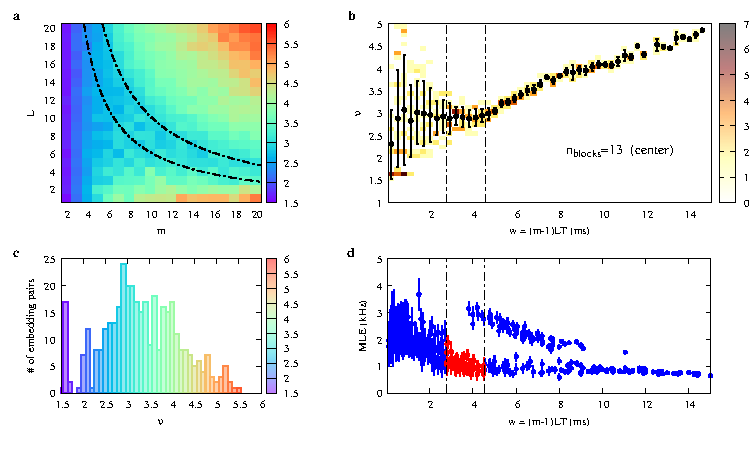
\includegraphics[width=\linewidth]{../blocks/13_blocks/middle/2e5_points/plots/chaos_low.pdf}
    \caption{``Chasing chaos'' analysis of the experimental $W_7$ time series with 13 coupled blocks.
    (a) Map of estimated correlation dimension $\nu$ vs.\ embedding pair $(m, L)$.
    (b) Sample joint distribution of $(w,\nu)$ for the $\nu$-map in (a).
    (c) Histogram of the estimated $\nu$. (d) Distribution of MLE as a function of $w$.
    }\label{fig: 13 blocks chaos center}
\end{figure}

In both cases, the various MLE points in the uniformity region are subdivided in two different clusters\footnote{
For the analysis, only the most populated clusters, i.e.\ the ones highlighted in red in the plots,
were considered.}.
This hints at the possiblity that there is more than one positive Lyapunov exponent in the system.
Since the divergence rate method is optimal when dealing with only one positive exponent,
it is likely that a systematic error of the method occurs.

In any case, the two plateaux for the boundary and center case are, respectively,
$\text{MLE}_\text{boundary}=865$ Hz and $\text{MLE}_\text{center}=1361$ Hz.
The MLE can then be estimated, in a simplistic manner, as the average between
these values, i.e.\ $\text{MLE}=(1.11\pm0.25)$ kHz, where the error is simply given by half of the difference
between $\text{MLE}_\text{boundary}$ and $\text{MLE}_\text{center}$.
The systematic error on this estimate
is not negligible and is indeed a big limit of the divergence rate method.
However, this value of MLE is meaningful, since the characteristic time of the circuit
(see Fig.~\ref{fig: circuit diagram}) is given by $\tau=RC=1$ ms; therefore, the characteristic
frequency of the circuit is 1 kHz, which complies with our estimate of the MLE\@.






